\subsubsection{Main results}
% \label{sec:4.2:webarena-results}

\begin{table}[t!]
\vspace{-3mm}
\centering
\small
\caption{Task success rate on WebArena using \texttt{gpt-4}, and score breakdown on five website splits.}
\vspace{2mm}
\label{tab:webarena-results}
%
\begin{tabular}{l|c|ccccc|c}
\toprule
\multicolumn{1}{c|}{\bf Method} & {\bf Total SR} & {Shopping} & {CMS} & {Reddit} & {GitLab} & {Maps} & {\bf \# Steps} \\
\midrule
\dlrow \multicolumn{8}{c}{\it With human engineered workflows} \\
{*SteP \citep{sodhi2023heap}} & {33.0} & {\bf 37.0} & {24.0} & {\bf 59.0} & {\bf 32.0} & {30.0} & {-} \\
\midrule
\dlrow \multicolumn{8}{c}{\it Autonomous agent only} \\
{WebArena \citep{zhou2024webarena}} & {14.9} & {14.0} & {11.0} & {~6.0} & {15.0} & {16.0} & {-} \\
{AutoEval \citep{pan2024autonomous}} & {20.2} & {25.5} & {18.1} & {25.4} & {28.6} & {31.9} & {46.7} \\
{BrowserGym \citep{drouin2024workarena}} & {23.5} & {-} & {-} & {-} & {-} & {-} & {-} \\
{BrowserGym$_{\it ax-tree}$} & {15.0} & {17.2} & {14.8} & {20.2} & {19.0} & {25.5} & {~~7.9} \\
\midrule
% \textsc{AWM$_{\it rule}$ (ours)} & {\bf 35.6} & {33.2} & {\bf 30.2} & {50.9} & {30.8} & {40.5} & {~~6.3} \\
\textsc{AWM (ours)} & {35.5} & {30.8} & {29.1} & {50.9} & {31.8} & {\bf 43.3} & {\bf ~~5.9} \\
\bottomrule
\end{tabular}
\vspace{-4mm}
\end{table}


As shown in \autoref{tab:webarena-results}, our \awm achieves the best published results on WebArena, surpassing the BrowserGym baseline by $12.0$ absolute points and $51.1$\% relative increase in overall success rate. Notably, \awm also outperforms SteP, which uses strong domain-specific supervision from human-written workflows, by a $7.6$\% relative increase in overall success rate.
According to the breakdown on five websites, our \awm method substantially enhances the agent performance across all websites over the BrowserGym baseline, by $11.8$--$30.7$ absolute points, indicating its general applicability across varied domains and tasks.

Beyond task success, we also evaluate the average number of steps the agent takes to solve a task, as shown in the rightmost column in \autoref{tab:webarena-results}. \awm conducts about $2.0$ fewer steps per example than the BrowserGym baseline. Further compared to the Autoeval \citep{pan2024autonomous} method, which necessitates additional evaluation and refinement steps to solve tasks correctly, our \awm approach uses $40.8$ fewer steps on average. Both comparisons show that \awm obtains high success rates while maintaining efficient trajectories.



%%%%%%%%%

\begin{wrapfigure}[15]{r}{0.5\textwidth}
\vspace{-2mm}
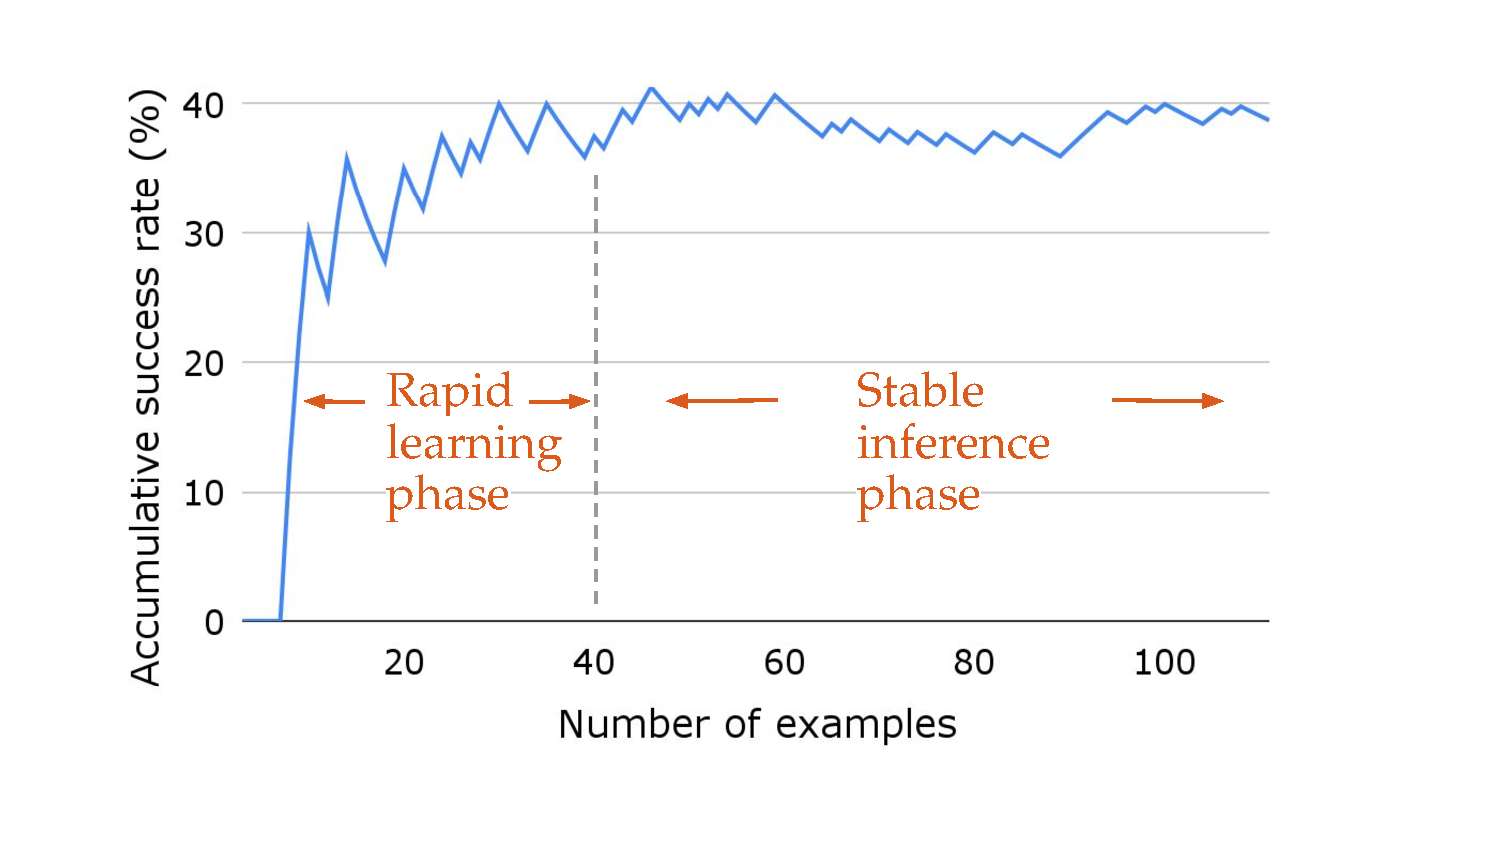
\includegraphics[width=0.49\textwidth]{./figures/webarena-learning.pdf}
% \vspace{-1mm}
\caption{\awm enables rapid learning from a small amount of data, i.e., about 40 queries, using WebArena map test split as an example.}
\label{fig:webarena-learning}
% \vspace{-1mm}
\end{wrapfigure}


%%%%%%%%%%
\subsubsection{Efficient learning from small amounts of data}
To demonstrate the behavior of the $\awm_{\it online}$ method, we illustrate the cumulative success rate over the process of online evaluation, by evaluating the average success rate of the first $k$ finished examples. 

As in \autoref{fig:webarena-learning}, the agent exhibits a fast learning curve in the beginning (between 0--40 examples), by acquiring the most essential workflows, which results in higher success rates. Afterward, agents learn more advanced workflows (\autoref{fig:teaser}), while success rates gradually stabilize to the highest point in the early learning phase.
This showcases \awm's efficient learning process, which substantially improves performance with merely tens of examples.



%%%%%%%%%%
\subsubsection{Cross-template workflow generalization}
Some tasks in the WebArena benchmark have highly overlapping canonical trajectories, due to the benchmark construction process that instantiates multiple examples from a single underlying task template. 
\awm intuitively improves in-template success rate, that is, given one workflow induced from a successful example, it would be theoretically easier to solve all other examples generated from the same task template.

To confirm that the benefits of \awm are not just from learning workflows that help only within a template, and investigate whether \awm can obtain cross-template ($\approx$cross-task) generalization, we extract a subset of WebArena examples sourcing from non-overlapping templates, by grouping examples by their templates and randomly choosing one example from each template group.
We run \awm on this cross-template subset and examine if it achieves similar performance gains.


\begin{table}[t!]
\vspace{-3mm}
\centering
\small
\caption{Task success rate on the cross-template subset of WebArena, as well as the result breakdown on each website split. We mark the number of examples for each website split under the name.}
\vspace{2mm}
\label{tab:cross-template-webarena-results}
%
\begin{tabular}{l|c|ccccc}
\toprule
\multicolumn{1}{c|}{\multirow{2}{*}{\bf Method}} & \multirow{2}{*}{\bf Total SR} & {Shopping} & {CMS} & {Reddit} & {GitLab} & {Maps} \\
{} & {} & {(51)} & {(45)} & {(24)} & {(45)} & {(32)} \\
\midrule
\dlrow \multicolumn{7}{c}{\it With human engineered workflows} \\
{*SteP \citep{sodhi2023heap}} & {32.1} & {\bf 26.5} & {\bf 29.3} & {\bf 52.2} & {27.3} & {36.4} \\
\midrule
\dlrow \multicolumn{7}{c}{\it Autonomous agent only} \\
{AutoEval \citep{pan2024autonomous}} & {23.2} & {12.2} & {17.1} & {21.7} & {\bf 31.8} & {36.4} \\
{BrowserGym$_{\it ax-tree}$} & {20.5} & {10.4} & {17.8} & {23.1} & {27.3} & {28.6} \\
\textsc{AWM (ours)} & {\bf 33.2} & {24.5} & {\bf 29.3} & {\bf 52.2} & {\bf 31.8} & {\bf 39.4} \\
\bottomrule
\end{tabular}
\vspace{-4mm}
\end{table}

As shown in \autoref{tab:cross-template-webarena-results}, \awm still achieves the highest performance, overall and on each website split. These results demonstrate that \awm induced workflows can effectively generalize across different tasks, i.e., examples instantiated from different task templates.


\begin{wrapfigure}[9]{r}{0.67\textwidth}
\vspace{-5mm}
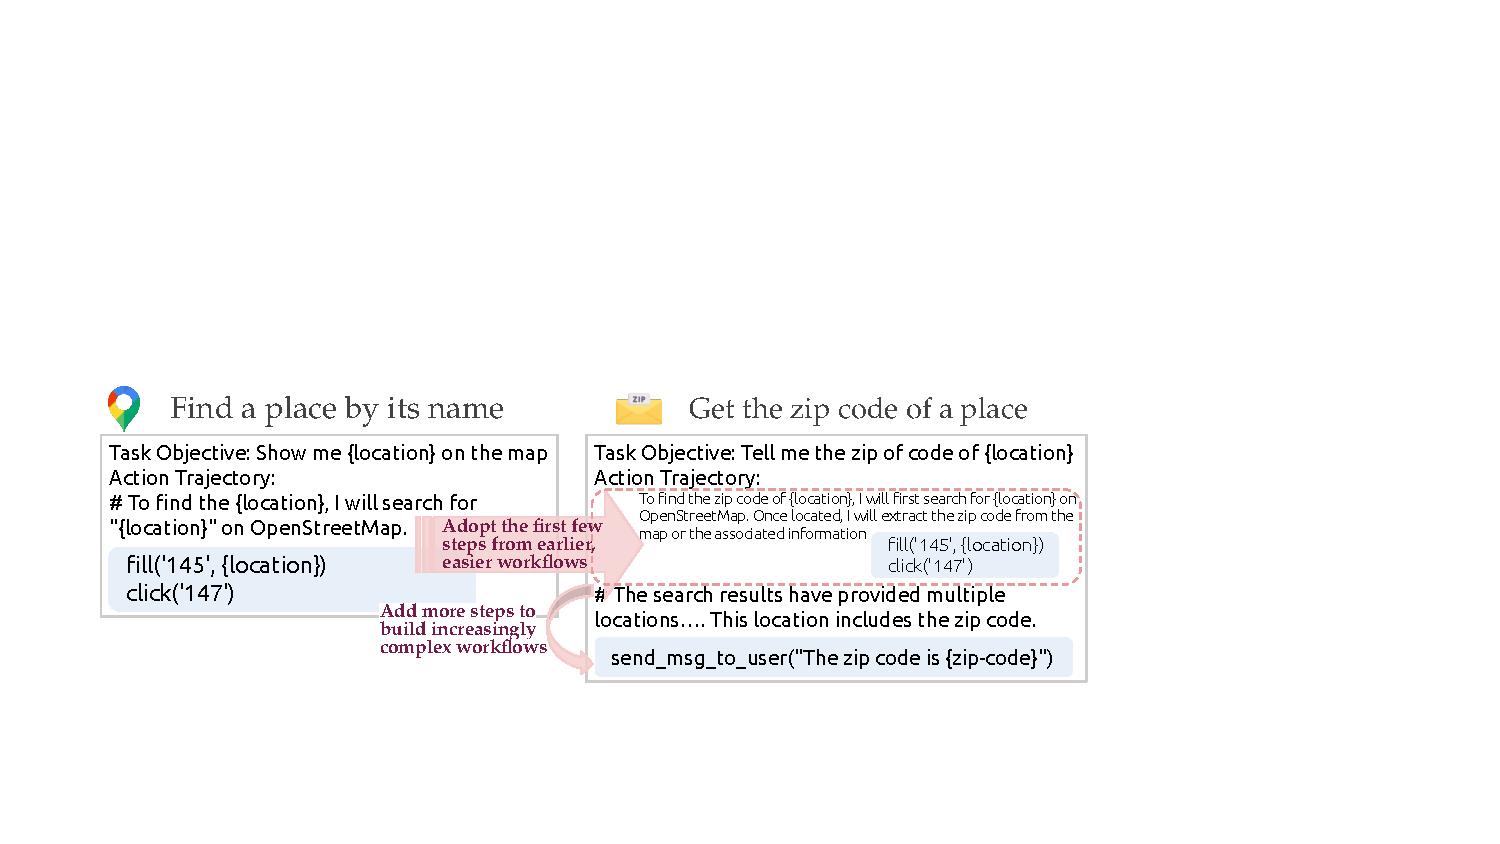
\includegraphics[width=0.67\textwidth]{./figures/complex-workflows.pdf}
\vspace{-6mm}
\caption{\awm builds increasingly complex workflows over time, by learning from past examples and earlier workflows.}
\label{fig:complex-workflows}
% \vspace{-1mm}
\end{wrapfigure}



% \noindent \textbf{Building increasingly complex workflows} \quad
\paragraph{Building increasingly complex workflows}
To more intuitively demonstrate \awm's cross-template generalization and ability to build increasingly complex workflows (as exemplified in \autoref{fig:teaser}), we conduct a case study to illustrate the workflow mechanism behind it. 

As exemplified in \autoref{fig:complex-workflows}, the agent creates and learns the ``Find a place by its name'' workflow in the early stage of the online process by summarizing past examples. Later, when encountering an example that further asks to obtain the zip code of the location, \awm agent learns to adopt the first few steps to find locations by following the existing workflow, and then conducts further steps to obtain the zip code of the place found. Integrating these new steps upon the vanilla find location task, the agent successfully builds a more complex workflow, i.e., ``get the zip code of a place''.
